\section{More with Integrals} \label{S:4.7.MoreIntegrals}

\begin{goals}
\item How can we use definite integrals to determine the average $y$-value of a function?
\item How can we use definite integrals to measure the area between two curves?
\item How do we decide whether to integrate with respect to $x$ or with respect to $y$ when we try to find the area of a region?
\end{goals} 

%-----------------------------------
% SUBSECTION INTRODUCTION
%-----------------------------------
\subsection*{Introduction}

Early in our work with the definite integral, we learned that if we have a nonnegative velocity function, $v$, for an object moving along an axis, the area under the velocity function between $a$ and $b$ tells us the distance the object traveled on that time interval.  Moreover, based on the definition of the definite integral, that area is given precisely by $\int_a^b v(t) \, dt$.  Indeed, for any nonnegative function $f$ on an interval $[a,b]$, we know that $\int_a^b f(x) \, dx$ measures the area bounded by the curve and the $x$-axis between $x = a$ and $x = b$.

In this section, we will further explore definite integrals including some important properties of integrals.  In Preview Activity~\ref{PA:4.7}, we begin this investigation with a refresher of certain contexts. 

\begin{pa} \label{PA:4.7}  Consider the following test scores of a particular student.
\[ 83, \enskip 75, \enskip 92, \enskip 68 \]

\ba
\item Calculate the student's average test score.
\item Would the method used in (a) to determine the average score change depending on the number of tests?
\item Is it necessarily the case that the student's average test score must equal exactly one of their actual test scores? Why or why not?
\ea

\noindent Consider a circle of radius $5$ and a square of side length $2$.

\ba
\item Compute the areas of the circle and square.
\item Suppose the square is placed wholly inside the circle.  How would you compute the area of the region inside the circle but outside the square?  What is the area of that region?
\ea
\end{pa} 
\afterpa % PREVIEW ACTIVITY Change activity or the order of the section

%-----------------------------------------------------------------
% SUBSECTION THE AVERAGE VALUE OF A FUNCTION
%-----------------------------------------------------------------
\subsection*{The Average Value of a Function}\index{average value of a function}

One of the most valuable applications of the definite integral is that it provides a way to meaningfully discuss the average value of a function, even for a function that takes on infinitely many values.  Suppose we wish to take the average of $n$ numbers $y_1$, $y_2$, $\ldots$, $y_n$.  We do so by computing
\[ \mbox{Avg} = \frac{y_1 + y_2 + \cdots + y_n}{n}. \]

Since integrals arise from Riemann sums in which we add $n$ values of a function, it should not be surprising that evaluating an integral is something like averaging the output values of a function.  Consider, for instance, the right Riemann sum $R_n$ of a function $f$, which is given by
\begin{align*}
R_n & = f(x_1) \triangle x + f(x_2) \triangle x + \cdots + f(x_n) \triangle x \\
& = \left( f(x_1) + f(x_2) + \cdots + f(x_n) \right) \triangle x.
\end{align*}
Since $\triangle x = \frac{b-a}{n}$, we can thus write 
\begin{align} \label{E:RAvg}
R_n &  = (f(x_1) + f(x_2) + \cdots + f(x_n))\cdot \frac{b-a}{n} \notag \\
& = (b-a) \frac{f(x_1) + f(x_2) + \cdots + f(x_n)}{n}.
\end{align}
Here, we see that the right Riemann sum with $n$ subintervals is the length of the interval $(b-a)$ times the average of the $n$ function values found at the right endpoints.  And just as with our efforts to compute area, we see that the larger the value of $n$ we use, the more accurate our average of the values of $f$ will be.  Indeed, we will define the average value of $f$ on $[a,b]$ to be 
\[ f_{\mbox{\tiny{AVG}}[a,b]} = \lim_{n \to \infty} \frac{f(x_1) + f(x_2) + \cdots + f(x_n)}{n}.\]  
But we also know that for any continuous function $f$ on $[a,b]$, taking the limit of a Riemann sum leads precisely to the definite integral.  That is, $\ds \lim_{n \to \infty} R_n = \int_a^b f(x) \, dx$, and thus taking the limit as $n \to \infty$ in Equation~(\ref{E:RAvg}), we have that
\begin{equation} \label{E:RAvg2} % EQUATION
\int_a^b f(x) \, dx = (b-a) \cdot f_{\mbox{\tiny{AVG}}[a,b]}.
\end{equation}
Solving Equation~(\ref{E:RAvg2}) for $f_{\mbox{\tiny{AVG}}[a,b]}$, we have the following general principle.

\concept{Average Value of a Function} % CONCEPT
{If $f$ is a continuous function on $[a,b]$, then its average value on $[a,b]$ is given by the formula
\[ f_{\mbox{\tiny{AVG}}[a,b]} = \frac{1}{b-a} \cdot \int_a^b f(x) \, dx. \]
} % end concept

\begin{marginfigure} % MARGIN FIGURE
\captionsetup[subfigure]{labelformat=empty}
\subfloat{\margingraphics{figs/4/4-7_AvgVala.pdf}}

\subfloat{\margingraphics{figs/4/4-7_AvgValb.pdf}}

\subfloat{\margingraphics{figs/4/4-7_AvgValc.pdf}}
\caption{A function $y = f(x)$, the area it bounds, and its average value on $[a,b]$.} \label{fig:4-7_AvgVal}
\end{marginfigure}

Observe that Equation~(\ref{E:RAvg2}) tells us another way to interpret the definite integral:  the definite integral of a function $f$ from $a$ to $b$ is the length of the interval $(b-a)$ times the average value of the function on the interval.  In addition, Equation~(\ref{E:RAvg2}) has a natural visual interpretation when the function $f$ is nonnegative on $[a,b]$.  

Consider Figure~\ref{fig:4-7_AvgVal}, where we see at the top the shaded region whose area is $\int_a^b f(x) \, dx$, in the middle the shaded rectangle whose dimensions are $(b-a)$ by $f_{\mbox{\tiny{AVG}}[a,b]}$, and at the bottom these two figures superimposed.  Specifically, note that in dark green we show the horizontal line $y = f_{\mbox{\tiny{AVG}}[a,b]}$.  Thus, the area of the green rectangle is given by $(b-a) \cdot f_{\mbox{\tiny{AVG}}[a,b]}$, which is precisely the value of $\int_a^b f(x) \, dx$.  Said differently, the area of the blue region in the top figure is the same as that of the green rectangle in the middle figure; this can also be seen by observing that the areas $A_1$ and $A_2$ in the bottom figure appear to be equal.  Ultimately, the average value of a function enables us to construct a {\em single} rectangle whose area is the same as the value of the definite integral of the function on the interval.  

The java applet at \href{http://gvsu.edu/s/az}{\texttt{http://gvsu.edu/s/az}} provides an opportunity to explore how the average value of the function changes as the interval changes, through an image similar to that found in Figure~\ref{fig:4-7_AvgVal}.

\begin{activity} \label{A:4.7.av}  Suppose that $\ds v(t) = \sqrt{4-(t-2)^2}$ tells us the instantaneous velocity of a moving object on the interval $0 \le t \le 4$, where $t$ is measured in minutes and $v$ is measured in meters per minute.
\ba
\item Sketch an accurate graph of $y = v(t)$.  What kind of curve is $\ds y = \sqrt{4-(t-2)^2}$?
\item Evaluate $\ds \int_0^4 v(t) \, dt$.
\item In terms of the physical problem of the moving object with velocity $v(t)$, what is the meaning of $\ds \int_0^4 v(t) \, dt$?  Include units on your answer.
\item Determine the exact average value of $v(t)$ on $[0,4]$.  Include units on your answer.
\item Sketch a rectangle whose base is the line segment from $t=0$ to $t = 4$ on the $t$-axis such that the rectangle's area is equal to the value of $\ds \int_0^4 v(t) \, dt$.  What is the rectangle's exact height?
\item How can you use the average value you found in (d) to compute the total distance traveled by the moving object over $[0,4]$?
\ea
\end{activity}
\begin{smallhint}
\ba
	\item Note that $y = \sqrt{4-(t-2)^2}$ is part of the curve given by $(t-2)^2 + y^2 = 4$.
	\item What familiar shape is generated by the curve $y = v(t)$?
	\item Recall the meaning of the area bounded by a nonnegative velocity function on a given interval.
	\item From the meaning of the average value of a function, we know $v_{\mbox{\tiny{AVG}}}[a,b] = \frac{1}{b-a}  \int_a^b v(t) \, dt$.
	\item Consider a key recent figure in the text.
	\item Distance equals average rate times $\ldots$.
\ea
\end{smallhint}
\begin{bighint}
\ba
	\item Note that $y = \sqrt{4-(t-2)^2}$ is the top half of the curve given by $(t-2)^2 + y^2 = 4$, which is a familiar one.
	\item What familiar shape is generated by the curve $y = v(t)$?  What known formula for area helps?
	\item Recall the meaning of the area bounded by a nonnegative velocity function on a given interval.  See, for instance, Section~\ref{S:4.1.VelocityDistance}.
	\item From the meaning of the average value of a function, we know $v_{\mbox{\tiny{AVG}}}[a,b] = \frac{1}{b-a}  \int_a^b v(t) \, dt$.  What are $a$ and $b$ in this problem?
	\item Consider a key recent figure in the text and construct a similar drawing for the given function $v$.
	\item Distance equals average rate times time!
\ea
\end{bighint}
\begin{activitySolution}
\ba
	\item The curve $y = v(t) = \sqrt{4-(t-2)^2}$ is the top half of the circle $(t-2)^2 + y^2 = 4$, which has radius 2 and is centered at $(2,0)$.
	\item Thus, the value of $\int_0^4 v(t) \, dt$ is the area of a semicircle of radius 2, which is $\frac{1}{2} \pi (2)^2 = 2\pi$.
	\item Because the velocity $v(t)$ is always nonnegative in this problem, the meaning of $\int_0^4 v(t) \, dt = 2\pi$ is both the distance traveled and the change in position of the object on the interval $0 \le t \le \pi$.  Specifically, the object moved $2 \pi$ meters in 4 minutes.
	\item We know $v_{\mbox{\tiny{AVG}}}[a,b] = \frac{1}{b-a}  \int_a^b v(t) \, dt$, so
	$$v_{\mbox{\tiny{AVG}}}[0,4] = \frac{1}{4-0}  \int_0^4 \sqrt{4-(t-2)^2} \, dt = \frac{1}{4} 2\pi = \frac{\pi}{2},$$
	which is measured in meters per minute, since the units on ``4'' are minutes and on ``$2\pi$'' are meters.
	\item Constructing a figure similar to those shown in this section on the topic of average value of a function, we find the following, which demonstrates a rectangle having the same area as the semicircle.
	\begin{center}
	  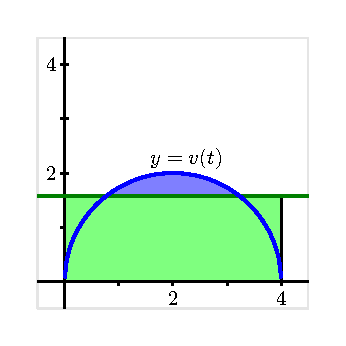
\includegraphics{figures/4_3_Act3Soln.eps}
	\end{center}
	The height of the rectangle is the average value of $v$, specifically $v_{\mbox{\tiny{AVG}}}[0,4] = \frac{\pi}{2} \approx 1.57$.
	\item Knowing that average velocity is $\frac{\pi}{2}$, it follows from the fact that distance traveled equals average rate times time (provided velocity is always nonnegative), we have
	$$D = \frac{\pi}{2} \cdot 4 = 2\pi.$$
	We see from (c) or (f) that we are simply considering the situation from two different perspectives: if we know the distance traveled, we can find average velocity, or if we know average velocity, we can find distance traveled.
\ea
\end{activitySolution}
\aftera





 % ACTIVITY

%----------------------------------------------------------------------------
% SUBSECTION THE MEAN VALUE THEOREM FOR INTEGRALS
%----------------------------------------------------------------------------
\subsection*{The Mean Value Theorem for Integrals}

The average value of a function brings us to an important theoretical result.  The Mean Value Theorem for Integrals says that if $f$ is continuous on the interval $[a,b]$, then there exists at least one point $c$ in the interval $[a,b]$ such that $f(c)$ equals the average value of $f$ on $[a,b]$.  In other words, the horizontal line $y = f_{\mbox{\tiny{AVG}}[a,b]}$ intersects the graph of $f$ for some point $c$ in $[a,b]$, or over the interval $[a,b]$, the average value of a function $f$ must equal its actual value at least once.\footnote{Compare this statement to the Mean Value Theorem for Derivatives, which says that over the interval $[a,b]$ the instantaneous rate of change of some function must equal its average rate of change at least once.}

\concept{Mean Value Theorem for Integrals}
{Let $f$  be continuous on the interval $[a,b]$.  There exists a point $c$ in $[a,b]$ such that
\[ f(c) = \frac{1}{b-a} \int_a^b f(x) \ dx. \]
} % end concept

\proof We begin by letting $F(x) = \int_a^x f(t) \ dt$ and noticing that $F$ is continuous on the interval $[a,b]$ and differentiable on the interval $(a,b)$ by the Fundamental Theorem of Calculus.  Applying the Mean Value Theorem for Derivatives to $F$, we can conclude that there exists at least one point $c$ in $(a,b)$ such that
\[ F'(c) = f(c) = \frac{F(b) - F(a)}{b-a}. \]
By the FTCII, we know that $F(b) - F(a)$ equals $\int_a^b f(x) \ dx$, so we can write
\[ f(c) = \frac{1}{b-a} \cdot F(b) - F(a) = \frac{1}{b-a} \int_a^b f(x) \ dx \]
where $c$ is some point in the interval $(a,b)$.
\qed

%----------------------------------------------------
% SUBSECTION AREA BETWEEN TWO CURVES
%----------------------------------------------------
\subsection*{The Area Between Two Curves} \index{area}

In Preview Activity~\ref{PA:4.7}, we encountered a notion that extends to area between two curves:  we can subtract the area of one region from the area of another to calculate the area ``between'' the regions.

\begin{marginfigure}[2cm] % MARGIN FIGURE
\captionsetup[subfigure]{labelformat=empty}
\subfloat{\margingraphics{figs/4/4-7_ABCa.pdf}}

\subfloat{\margingraphics{figs/4/4-7_ABCb.pdf}}

\subfloat{\margingraphics{figs/4/4-7_ABCc.pdf}}
\caption{The areas bounded by the functions $f(x) = (x-1)^2 + 1$ and $g(x) = x+2$ on the interval $[0,3]$.} \label{fig:4-7_ABC}
\end{marginfigure}

For the functions $f(x) = (x-1)^2 + 1$ and $g(x) = x+2$, shown in Figure~\ref{fig:4-7_ABC}, we see that the upper curve is $g(x) = x+2$, and that the graphs intersect at $x = 0$ and $x=3$.  Note that we can find where these functions intersect by setting the functions equal to each other and solving for $x$:
\begin{align*}
f(x) & = g(x) \\
(x-1)^2 + 1 & = x+2 \\
x^2 - 2x +2 & = x+2 \\
x^2 - 3x & = 0 \\
x(x-3) & = 0 \\
\Rightarrow x &= 0,3.
\end{align*}
On the interval $[0,3]$, the area beneath $g$ is
\[ \int_0^3 (x+2) \, dx = \frac{21}{2}, \]
while the area under $f$ on the same interval is
\[ \int_0^3 [(x-1)^2 + 1] \, dx = 6. \]
Thus, the area between the curves is 
\begin{equation} \label{E:DiffOfInt} % EQUATION
A = \int_0^3 (x+2) \, dx -  \int_0^3 [(x-1)^2 + 1] \, dx = \frac{21}{2} - 6 = \frac{9}{2}.
\end{equation}

\begin{marginfigure} % MARGIN FIGURE
\margingraphics{figs/4/4-7_ABCd.pdf}
\caption{The area bounded by the functions $f(x) = (x-1)^2 + 1$ and $g(x) = x+2$ on the interval $[0,3]$.} 
\label{fig:4-7_ABCd}
\end{marginfigure}

A slightly different perspective is also helpful here:  if we take the region between two curves and slice it up into thin vertical rectangles (in the same spirit as we originally sliced the region between a single curve and the $x$-axis in Section~\ref{S:4.2.Riemann}), then we see that the height of a typical rectangle is given by the difference between the two functions.  For example, for the rectangle shown in Figure~\ref{fig:4-7_ABCd}, we see that the rectangle's height is $g(x) - f(x)$, while its width can be viewed as $\triangle x$, and thus the area of the rectangle is
\[ A_{\mbox{\small{rect}}} = (g(x) - f(x)) \triangle x. \]
In addition, the area between the two curves on the interval $[0,3]$ is then approximated by the Riemann sum
\[ A \approx \sum_{i=1}^{n} (g(x_i) - f(x_i)) \triangle x, \]
and then as we let $n \to \infty$, it follows that the area is given by the single definite integral
\begin{equation} \label{E:IntOfDiff} % EQUATION 
A = \int_0^3 (g(x) - f(x)) \, dx.
\end{equation}
In our work with applications of the definite integral, we will often find it helpful to think of a ``representative slice'' and how the definite integral may be used to add these slices to find the exact value of a desired quantity.  Here, the integral essentially sums the areas of thin rectangles.

Also, we note that whether we think of the area between two curves as stemming from the difference between the area bounded by the individual curves (as in Equation~(\ref{E:DiffOfInt})) or as the limit of a Riemann sum that adds the areas of thin rectangles between the curves (as in Equation~(\ref{E:IntOfDiff})), these two results are the same, since the difference of two integrals is the integral of the difference:
\[ \int_0^3 g(x) \, dx -  \int_0^3 f(x) \ dx = \int_0^3 (g(x) - f(x)) \ dx. \]

Finally, notice that if we had computed
\[ \int_0^3 (f(x) - g(x)) \ dx \mbox{ instead of } \int_0^3 (g(x) - f(x)) \ dx, \]
then our result would have been $\ds -\frac{9}{2}$, which has the same magnitude as the correct result, but the sign is negative.  Whereas the net signed area underneath a function can be either positive or negative, the area that is bounded by or between two curves will be positive.  Therefore, we can simply take the absolute value of our negative result to get the correct result, leading to the following concept.

\concept{Area Between Curves} % CONCEPT 
{If two curves $y = f(x)$ and $y = g(x)$ intersect only at $x=a$ and $x=b$ on $[a,b]$, then the area between the curves on the interval $[a,b]$ is 
\[ A = \left| \int_a^b (f(x) - g(x)) \ dx \right|. \]
} % end concept

\begin{example} % EXAMPLE
Find the area of the region bounded by $y=x^2+x-5$ and $y=3x-2$.

\solution We begin by finding the $x$-values at which the functions intersect. 
\begin{align*} x^2+x-5 &= 3x-2 \\
(x^2+x-5) - (3x-2) &= 0\\
x^2-2x-3 &= 0\\
(x-3)(x+1) &= 0\\
x&=-1,\ 3.
\end{align*}
Therefore, the area is 
\begin{align*}
\int_{-1}^3\big(3x-2 -(x^2+x-5)\big)\ dx &= \int_{-1}^3 (-x^2+2x+3)\ dx \\
&=\left.\left(-\frac13x^3+x^2+3x\right)\right|_{-1}^3 \\
&=-\frac{27}{3}+9+9-\left(\frac13+1-3\right)\\
&= \frac{32}{3}.
\end{align*}
\end{example} % EXAMPLE

\begin{activity} \label{A:4.4.2}  In each of the following problems, our goal is to determine the area of the region described.  For each region, (i) determine the intersection points of the curves, (ii) sketch the region whose area is being found, (iii) draw and label a representative slice, and (iv) state the area of the representative slice.  Then, state a definite integral whose value is the exact area of the region, and evaluate the integral to find the numeric value of the region's area.
\ba
	\item The finite region bounded by $y = \sqrt{x}$ and $y = \frac{1}{4}x$.
	\item The finite region bounded by $y = 12-2x^2$ and $y = x^2 - 8$.
	\item The area bounded by the $y$-axis, $f(x) = \cos(x)$, and $g(x) = \sin(x)$, where we consider the region formed by the first positive value of $x$ for which $f$ and $g$ intersect.
	\item The finite regions between the curves $y = x^3-x$ and $y = x^2$.
\ea
\end{activity}
\begin{smallhint}
\ba
	\item Small hints for each of the prompts above.
\ea
\end{smallhint}
\begin{bighint}
\ba
	\item Big hints for each of the prompts above.
\ea
\end{bighint}
\begin{activitySolution}
\ba
	\item Solutions for each of the prompts above.
\ea
\end{activitySolution}
\aftera % ACTIVITY

%-----------------------------------------------------------------------
% SUBSECTION FINDING AREA WITH HORIZONTAL SLICES
%-----------------------------------------------------------------------
\subsection*{Finding Area with Horizontal Slices}

At times, the shape of a geometric region may dictate that we need to use horizontal rectangular slices, rather than vertical ones.  For instance, consider the region bounded by the parabola $x = y^2 - 1$ and the line $y = x-1$, pictured in Figure~\ref{fig:4-7_ABCe}.  First, we observe that by solving the second equation for $x$ and writing $x = y + 1$, we can then determine the $y$-values at which the curves intersect by again setting the curves equal to each other and solving for $y$:
\begin{align*}
y^2 - 1 & = y+1 \\
y^2 - y - 2 &= 0 \\
(y-2)(y+1) &= 0 \\
\Rightarrow y &= -1,2.
\end{align*}

\begin{marginfigure}[-6cm] % MARGIN FIGURE
\margingraphics{figs/4/4-7_ABCe.pdf}
\caption{The area bounded by the functions $x = y^2-1$ and $y = x-1$.} 
\label{fig:4-7_ABCe}
\end{marginfigure}

We can use the $y$-values to determine the $x$-values at which the curves intersect, which are $x=0$ and $x=3$. We see that if we attempt to use vertical rectangles to slice up the area, at certain values of $x$ (specifically from $x = -1$ to $x = 0$, as seen in Figure~\ref{fig:4-7_ABCf}), the curves that govern the top and bottom of the rectangle are one and the same.  This suggests, as shown in Figure~\ref{fig:4-7_ABCg}, that we try using horizontal rectangles as a way to think about the area of the region.

\begin{marginfigure}
\margingraphics{figs/4/4-7_ABCf.pdf}
\caption{The area bounded by the functions $x = y^2-1$ and $y = x-1$ with the region sliced vertically.} 
\label{fig:4-7_ABCf}
\end{marginfigure}

For such a horizontal rectangle, note that its width depends on $y$, the height at which the rectangle is constructed.  In particular, at a height $y$ between $y = -1$ and $y = 2$, the right end of a representative rectangle is determined by the line, $x = y+1$, while the left end of the rectangle is determined by the parabola, $x = y^2-1$, and the thickness of the rectangle is $\triangle y$.  

\begin{marginfigure}
\margingraphics{figs/4/4-7_ABCg.pdf}
\caption{The area bounded by the functions $x = y^2-1$ and $y = x-1$ with the region sliced horizontally.} 
\label{fig:4-7_ABCg}
\end{marginfigure}

Therefore, the area of the rectangle is
\[ A_{\mbox{\small{rect}}} = [(y+1) - (y^2-1)] \triangle y, \]
from which it follows that the area between the two curves on the $y$-interval $[-1,2]$ is approximated by the Riemann sum
\[ A \approx \sum_{i=1}^{n} [(y_i+1)-(y_i^2-1)] \triangle y.\]
Taking the limit of the Riemann sum, it follows that the area of the region is
\begin{equation} \label{E:IntWRTy} % EQUATION
A = \int_{y=-1}^{y=2} [(y+1) - (y^2-1)] \, dy.
\end{equation}
We emphasize that we are integrating with respect to $y$; this is dictated by the fact that we chose to use horizontal rectangles whose widths depend on $y$ and whose thickness is denoted $\triangle y$.  It is a straightforward exercise to evaluate the integral in Equation~(\ref{E:IntWRTy}) and find that $A = \frac{9}{2}$.

Just as with the use of vertical rectangles of thickness $\triangle x$, we have a general principle for finding the area between two curves, which we state as follows.

\concept{Area Between Curves}
{If two curves $x = f(y)$ and $x = g(y)$ intersect only at $y=c$ and $y=d$ on $[c,d]$, then the area between the curves on the interval $[c,d]$ is 
\[ A = \left| \int_{y=c}^{y=d} (f(y) - g(y)) \ dy \right|. \]
} % end concept

\begin{activity} \label{A:4.7.3}  In each of the following problems, our goal is to determine the area of the region described.  For each region, 
\begin{enumerate}[(i),leftmargin=*]
\item determine the intersection points of the curves,
\item sketch the region whose area is being found,
\item draw and label a representative slice, and
\item state the area of the representative slice.
\end{enumerate}
Then, state a definite integral whose value is the exact area of the region, and evaluate the integral to find the numeric value of the region's area.  {\bf Note well:} At the step where you draw a representative slice, you need to make a choice about whether to slice vertically or horizontally.
\ba
	\item The finite region bounded by $x=y^2$ and $x=6-2y^2$.
	\item The finite region bounded by $x=1-y^2$ and $x = 2-2y^2$.
	\item The area bounded by the $x$-axis, $y=x^2$, and $y=2-x$.
	\item The finite regions between the curves $x=y^2-2y$ and $y=x$.

\ea

\end{activity}
\begin{smallhint}
\ba
	\item Small hints for each of the prompts above.
\ea
\end{smallhint}
\begin{bighint}
\ba
	\item Big hints for each of the prompts above.
\ea
\end{bighint}
\begin{activitySolution}
\ba
	\item Solutions for each of the prompts above.
\ea
\end{activitySolution}
\aftera

\begin{summary}
\item The definite integral $\int_a^b f(x) \,dx$ measures the exact net signed area bounded by $f$ and the horizontal axis on $[a,b]$; in addition, the value of the definite integral is related to what we call the average value of the function on $[a,b]$: $f_{\mbox{\tiny{AVG}}[a,b]} = \frac{1}{b-a} \cdot \int_a^b f(x) \, dx.$  

\item To find the area between two curves, we think about slicing the region into thin rectangles.  If, for instance, the area of a typical rectangle on the interval $x = a$ to $x = b$ is given by $A_{\mbox{\small{rect}}} = (g(x) - f(x)) \triangle x,$ then the exact area of the region is given by the definite integral
\[ A = \int_a^b (g(x)-f(x))\, dx. \]

\item The shape of the region usually dictates whether we should use vertical rectangles of thickness $\triangle x$ or horizontal rectangles of thickness $\triangle y$.  We desire to have the height of the rectangle governed by the difference between two curves:  if those curves are best thought of as functions of $y$, we use horizontal rectangles, whereas if those curves are best viewed as functions of $x$, we use vertical rectangles.
\end{summary}

%--------------
% EXERCISES
%--------------
\begin{adjustwidth*}{}{-2.25in}
\textbf{{\large Exercises}}
\setlength{\columnsep}{25pt}
\begin{multicols*}{2}
\noindent {\normalsize Problems} \small

\noindent{\bf In exercises 1--7, find the average value of the function on the given interval.}

\begin{enumerate}[1)]
\item $f(x)=\sin(x)$ on $[0,\pi/2]$
\item $y=\sin(x)$ on $[0,\pi]$
\item $y=x$ on $[0,4]$
\item $\ds f(x) = \frac{1}{1+x^2}$ on $[1,\sqrt{3}]$
\item $y=x^3$ on $[0,4]$
\item $g(t) = 1/t$ on $[1,e]$
\item $f(x) = \sec^2(x)$ on $[-\pi/4, \pi/4]$
\end{enumerate}

\noindent{\bf In exercises 8--11, find a value $c$ guaranteed by the Mean Value Theorem.}

\begin{enumerate}[1),resume]
\item $\ds \int_0^2 x^2\ dx$
\item $\ds \int_{-2}^2 x^2\ dx$
\item $\ds \int_{0}^1 e^x\ dx$
\item $\ds \int_{0}^{16} \sqrt{x}\ dx$
\end{enumerate}

\noindent{\bf In exercises 12--14, find the area of the shaded region in each given figure.}

\bmtwo
\begin{enumerate}[1),resume]
\item \noindent
\begin{minipage}{\linewidth}
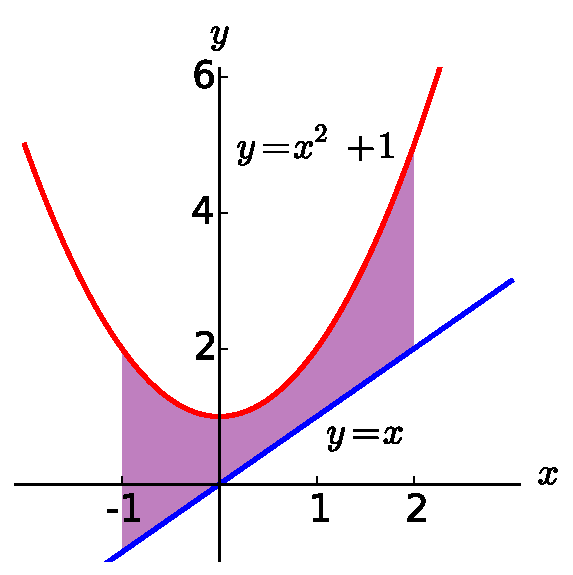
\includegraphics[scale=.35]{figs/4/4-7_Exa.pdf}
\end{minipage}

\item \noindent
\begin{minipage}{\linewidth}
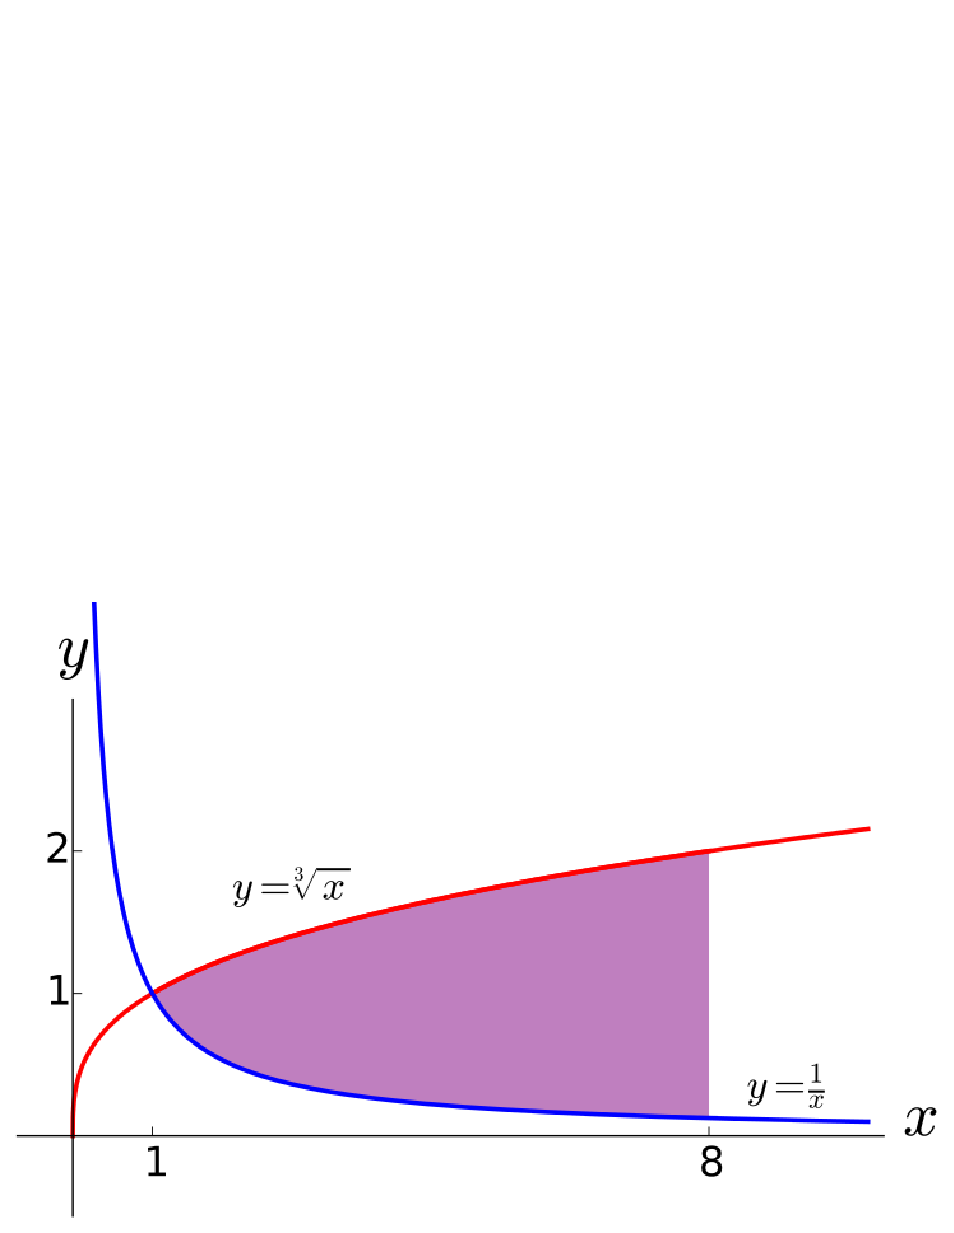
\includegraphics[scale=.35]{figs/4/4-7_Exc.pdf}
\end{minipage}

\item \noindent
\begin{minipage}{\linewidth}
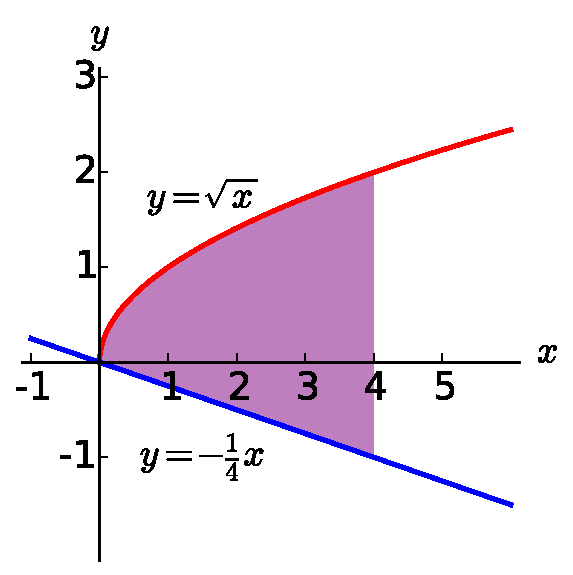
\includegraphics[scale=.35]{figs/4/4-7_Exb.pdf}
\end{minipage}
\end{enumerate}
\emtwo

\noindent{\bf In exercises 15--21, sketch the given functions and find the area of the enclosed region.}

\begin{enumerate}[1),start=15]
\item $y=2x$, $y=5x$, and $x= 3$.
\item $y=-x+1$, $y=3x+6$, $x=2$ and $x= -1$.
\item $y=x^2-2x+5$ and $y=5x-5$.
\item $y=2x^2+2x-5$ and $y=x^2+3x+7$.
\item $y = \cos(x)$ and $y = 1 - \cos(x)$ on $[0,\pi]$
\item $x = 1 - y^2$ and $x = y^2 - 1$
\item $4x + y^2 = 12$ and $x = y$

\item Suppose that the value of a car in dollars after $t$ years of use is $V(t) = 45,000e^{-0.25t}$. What is the average value of the yacht over its first $8$ years of use?

\item Water is run at a constant rate of $3$ ft$^3$/min to fill a cylindrical tank of radius $4$ ft and height $6$ ft. Assuming that the tank is initially empty, determine the average weight of the water in the tank over the time period required to fill it. Take the weight density of water to be $62.4$ lb/ft$^3$.
\end{enumerate}

%------------------------------------------
% END OF EXERCISES ON FIRST PAGE
%------------------------------------------
\end{multicols*}
\end{adjustwidth*}

%\clearpage
%
%\begin{adjustwidth*}{}{-2.25in}
%\setlength{\columnsep}{25pt}
%\begin{multicols*}{2}\small
%
%\end{enumerate}
%
%%---------------------------------------------
%% END OF EXERCISES ON SECOND PAGE
%%---------------------------------------------
%\end{multicols*}
%\end{adjustwidth*}

\afterexercises 

\cleardoublepage